\section{Part II: Computational Scalability under Full Quasi-Newton Optimization (\texttt{RQ2-bis})}
\label{sec:rq2bis}

While \texttt{RQ2} established which reconstructor architectures can represent each PDE family at fixed dynamics capacity and a short 200 Adam + 500 BFGS budget, two fundamental questions remained open:
\begin{enumerate}[leftmargin=2em]
  \item In Case~B, where the 17-mode POD floor is $\NRMSE = 3.46\cdot 10^{-4}$ ($57\times$ below \texttt{RQ2}'s $\mathrm{L0}$ and $23\times$ below \texttt{RQ2}'s $\mathrm{L2}$), was the accuracy of end-to-end training bottlenecked by the tiny canonical dynamics network ($7\text{--}7\text{--}d_s$, having only $85$--$220$ parameters) or by the $500$-iteration BFGS cap?
  \item Across both smooth vortex flows (Case~B) and sharp travelling fronts (Case~C), how does the test error $\NRMSE(P_{\mathrm{dyn}}, L, n, \text{iterations})$ scale when the dynamics network width $w$, depth $L$, latent dimension $n$, and quasi-Newton iteration budget are scaled up to $10{,}000$ BFGS iterations?
\end{enumerate}

\subsection{Experimental Design and the CINECA Leonardo HPC Campaign}

To trace the complete surface $\mathrm{error}(P, \text{iterations})$ without confounding from a first-order learning-rate schedule or an arbitrary Adam-to-BFGS switch point, \texttt{RQ2-bis} removes the Adam warm-up (\texttt{epochs\_adam = 0}) and optimizes all models from Glorot initialization using pure \texttt{scipy} BFGS (\texttt{method='BFGS'}, \texttt{gtol=1e-100}, \texttt{maxiter=10000}). Because a deterministic quasi-Newton trajectory has no learning-rate schedule---its step at iteration $k$ depends exclusively on the current gradient and the inverse-Hessian approximation accumulated over steps $0,\dots,k-1$---a single run of $I_{\max} = 10{,}000$ iterations equipped with a passive observation hook (\texttt{callback\_extra}) at the nine logarithmic checkpoints
\begin{equation}
  k \in \{25,\, 50,\, 100,\, 200,\, 500,\, 1000,\, 2000,\, 5000,\, 10000\}
  \label{eq:checkpoints}
\end{equation}
is mathematically identical to nine independent training runs stopped at each $k$. The time spent evaluating validation and full-grid test metrics inside the checkpoint hook (\texttt{ck\_time}) is explicitly measured and subtracted from both \texttt{train\_time\_s} and the cumulative trajectory time \texttt{time\_s} in \texttt{curves.csv}.

In each benchmark (Case~B and Case~C), we run two end-to-end ($\mathrm{R2}$) reconstructor arms across 21 configurations $\times$ 3 seeds $= 63$ runs per case (126 runs in total):
\begin{itemize}[leftmargin=2em]
  \item \textbf{Main Arm ($\mathrm{L0}$, Stages 0--2, 10 configs $\times$ 3 seeds $= 30$ runs/case):} The original pointwise MLP reconstructor ($24^4\to 2$ with cubic link in Case~B; $17^5\to 1$ in Case~C), sweeping:
  \begin{enumerate}[label=(\alph*)]
    \item \emph{Dynamics hidden width} $w \in \{w^*/4, w^*/2, w^*, 2w^*, 4w^*\}$ at canonical depth $L^*$ and latent size $n^*$, namely $w \in \{2, 4, 7, 14, 28\}$ at $(L^*=2, n^*=1)$ in Case~B ($P_{\mathrm{dyn}} \in \{15, 37, 85, 267, 925\}$) and $w \in \{2, 4, 8, 16, 32\}$ at $(L^*=1, n^*=12)$ in Case~C ($P_{\mathrm{dyn}} \in \{66, 120, 228, 444, 876\}$);
    \item \emph{Dynamics hidden depth} $L \in \{1, 2, 3\}$ at canonical $(w^*, n^*)$;
    \item \emph{Latent dimension} $n \in \{1, 2, 5, 10\}$ in Case~B and $n \in \{3, 6, 12, 24\}$ in Case~C at canonical $(w^*, L^*)$.
  \end{enumerate}
  \item \textbf{Linear Reconstructor Arm ($\mathrm{L2}$, Stage 7, 11 configs $\times$ 3 seeds $= 33$ runs/case):} The strictly linear modal synthesis $\bar{y}(\mathbf{x}) + \sum_{k=1}^K (W\mathbf{z}+\mathbf{b})_k \varphi_k(\mathbf{x})$ on the vector POD basis (Case~B) or trapezoidal-QR Legendre basis (Case~C), sweeping:
  \begin{enumerate}[label=(\alph*)]
    \item \emph{Latent dimension} $n \in \{1, 2, 5, 10\}$ (Case~B) and $n \in \{3, 6, 12, 24\}$ (Case~C) at $K_{\mathrm{L2}} = 65$ and canonical $(w^*, L^*)$;
    \item \emph{Dynamics hidden width} $w \in \{2, 4, 7, 14, 28\}$ at $(n_{\mathrm{L2}}=10, K=65, L^*=2)$ in Case~B ($P_{\mathrm{dyn}} \in \{60, 118, 220, 528, 1438\}$) and $w \in \{2, 4, 8, 16, 32\}$ at $(n_{\mathrm{L2}}=12, K=65, L^*=1)$ in Case~C ($P_{\mathrm{dyn}} \in \{66, 120, 228, 444, 876\}$);
    \item \emph{Basis truncation size} $K \in \{5, 17, 33, 65\}$ at $(w^*, L^*, n_{\mathrm{L2}})$.
  \end{enumerate}
\end{itemize}

\paragraph{Two-Pass Hardware Execution on CINECA Leonardo.}
An initial $1{,}000$-iteration pilot campaign of all 126 runs on an Apple M5 Pro workstation (18 CPU cores, 48~GB unified memory, preserved in \texttt{results\_1000iters/}) revealed that at iteration $1{,}000$ the test NRMSE was still dropping by $25\%$ to $49\%$ over the last 500 iterations across nearly all $\mathrm{L0}$ configurations. We therefore raised the budget tenfold to \textbf{$I_{\max} = 10{,}000$ BFGS iterations} (matching the original paper's full Case~B BFGS budget and doubling its Case~C budget) and executed the production campaign on the \textbf{Data Centric General Purpose (\texttt{dcgp\_usr\_prod}) partition of the CINECA Leonardo supercomputer} (dual-socket Intel Xeon Platinum 8480+ ``Sapphire Rapids'' compute nodes, $2 \times 56 = 112$ physical CPU cores per node, Linux 4.18, Python 3.11.7, TensorFlow 2.13.1 in IEEE-754 \texttt{float64} precision).

To prevent multi-job node contention from contaminating wall-clock measurements, we enforced a strict two-pass protocol:
\begin{enumerate}[leftmargin=2em]
  \item \textbf{Pass A (Accuracy Sweeps):} Each case was partitioned across four Slurm array shards (\texttt{--array=0-3}, 56 cores per shard) via \texttt{RQ2BIS\_SHARD=i/4}, recording all weights, predictions, checkpoint trajectories, function/gradient evaluation counts $n_{\mathrm{fev}}$, and shared-node wall-times $T_{\mathrm{Pass\,A}}$, then merged via \texttt{cluster/merge\_results.py}.
  \item \textbf{Pass T (Exclusive-Node Timing and Thread Scaling, Stage 5):} Following Pass~A, we allocated one \textbf{exclusive} 112-core Leonardo compute node per case (\texttt{--exclusive}, node \texttt{lrdn4887} for Case~B, Slurm job \texttt{60616414}; node \texttt{lrdn4960} for Case~C, Slurm job \texttt{60616416}). Because TensorFlow locks its thread pool upon initialisation, \texttt{timing\_worker.py} spawns a fresh subprocess for each thread count $p \in \{1, 2, 4, 8, 16, 32, 64, 112\}$ (setting \texttt{OMP\_NUM\_THREADS = MKL\_NUM\_THREADS = OPENBLAS\_NUM\_THREADS = p} and TensorFlow's intra/inter-op threads to $p$ prior to import), loads the exact trained weights from \texttt{results/weights/}, performs a warm-up evaluation, and measures the median over 3 repeats of the mean of 20 joint loss-and-gradient evaluations ($s_{\mathrm{eval}}$). At the optimal operating point $p^* = 16$ threads, all 21 configurations of the case are timed in randomized order (\texttt{RandomState(0).permutation}), with the first configuration repeated at the end to verify absence of thermal or cluster throttling ($1.3\%$ drift in Case~B; $7.6\%$ in Case~C, both well within the $10\%$ protocol threshold). The uncontaminated \textbf{Pass-T training wall-time} of any run is then $T_{\mathrm{Pass\,T}} = n_{\mathrm{fev}} \times s_{\mathrm{eval}}$.
\end{enumerate}

\subsection{Case B Scalability Results: \texorpdfstring{$\mathrm{L0}$}{L0} Plateau vs.\ \texorpdfstring{$\mathrm{L2}$}{L2} Power-Law Scaling}

Table~\ref{tab:rq2bis_caseB} reports the complete results of all 21 configurations in Case~B at the $10{,}000$-iteration BFGS budget, and Figure~\ref{fig:rq2bis_fig1} (left column) shows the resulting capacity scaling curves against $P_{\mathrm{dyn}}$ and $P_{\mathrm{total}}$.

\begin{figure}[!htbp]
  \centering
  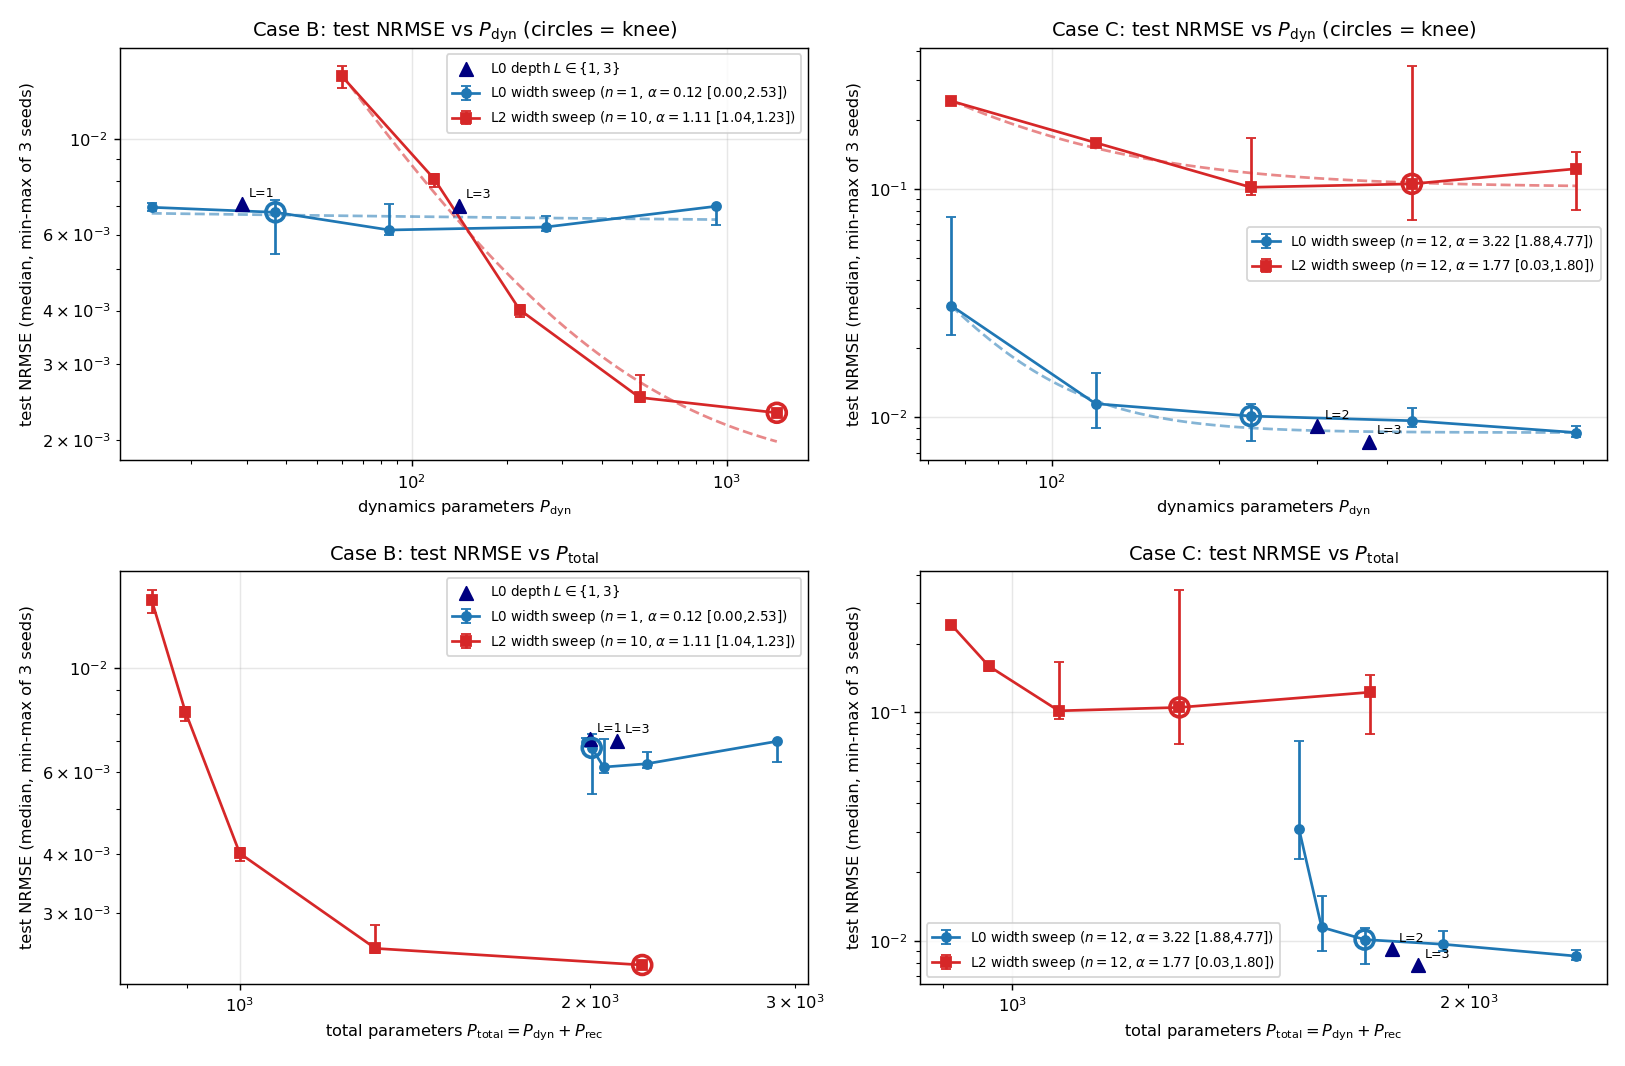
\includegraphics[width=0.90\textwidth,height=0.215\textheight,keepaspectratio]{fig1_capacity_laws.png}
  \caption{Stage~1 capacity scaling at the $10{,}000$-iteration BFGS budget on CINECA Leonardo: test NRMSE (median and min--max range over 3 seeds) against dynamics parameters $P_{\mathrm{dyn}}$ (\textbf{top row}, with fitted power laws $E(P_{\mathrm{dyn}}) = E_\infty + a\,P_{\mathrm{dyn}}^{-\alpha}$ dashed and validation-selected knees circled) and against total parameters $P_{\mathrm{total}} = P_{\mathrm{dyn}} + P_{\mathrm{rec}}$ (\textbf{bottom row}), for Case~B (\textbf{left}) and Case~C (\textbf{right}).}
  \label{fig:rq2bis_fig1}
\end{figure}

\begin{table}[!htbp]
\centering
\caption{Case B (\texttt{2D-Stokes}): all 21 configurations at the $10{,}000$-iteration BFGS budget on CINECA Leonardo (median and $[\min,\max]$ over 3 seeds). Here \texttt{st} is the number of early-stopped seeds out of 3, $s_{\mathrm{eval}}$ is the exclusive-node Pass-T evaluation time at 16 threads, $T_{\mathrm{Pass\,T}} = n_{\mathrm{fev}} s_{\mathrm{eval}}$, and $\eta = \varepsilon_{\mathrm{total}}/\varepsilon_{\mathrm{proj}}$. Bold rows mark the validation-selected best configuration of each arm.}
\label{tab:rq2bis_caseB}
\scriptsize
\setlength{\tabcolsep}{3.5pt}\resizebox{\textwidth}{!}{%

\begin{tabular}{@{}lrrrrrrrrrrrrrrlrr@{}}
\toprule
\textbf{Arm} & $K$ & $w$ & $L$ & $n$ & \textbf{st} & $P_{\mathrm{dyn}}$ & $P_{\mathrm{rec}}$ & $P_{\mathrm{tot}}$ & $\min\text{it}$ & $n_{\mathrm{fev}}$ & $s_{\mathrm{eval}}$[s] & $T_{\mathrm{PassT}}$[s] & $T_{\mathrm{PassA}}$[s] & \textbf{Valid} & \textbf{Test NRMSE $[\min,\max]$} & \textbf{Dir.} & \textbf{Vort.} \\
\midrule
L0 & $0$ & $2$ & $2$ & $1$ & $0$ & $15$ & $1970$ & $1985$ & $10000$ & $10042$ & $0.308$ & $3090$ & $4620$ & $5.84\cdot 10^{-3}$ & $6.94\cdot 10^{-3}$ $[6.82, 7.10]\cdot 10^{-3}$ & $0.0214$ & $0.389$ \\
L0 & $0$ & $4$ & $2$ & $1$ & $0$ & $37$ & $1970$ & $2007$ & $10000$ & $10042$ & $0.315$ & $3160$ & $4840$ & $5.65\cdot 10^{-3}$ & $6.76\cdot 10^{-3}$ $[5.40, 7.23]\cdot 10^{-3}$ & $0.0208$ & $0.358$ \\
L0 & $0$ & $7$ & $1$ & $1$ & $0$ & $29$ & $1970$ & $1999$ & $10000$ & $10044$ & $0.312$ & $3130$ & $4900$ & $5.92\cdot 10^{-3}$ & $7.06\cdot 10^{-3}$ $[6.86, 7.44]\cdot 10^{-3}$ & $0.0219$ & $0.429$ \\
L0 & $0$ & $7$ & $2$ & $1$ & $0$ & $85$ & $1970$ & $2055$ & $10000$ & $10050$ & $0.313$ & $3140$ & $4910$ & $5.27\cdot 10^{-3}$ & $6.15\cdot 10^{-3}$ $[5.98, 7.07]\cdot 10^{-3}$ & $0.0209$ & $0.312$ \\
L0 & $0$ & $7$ & $2$ & $2$ & $0$ & $100$ & $1994$ & $2094$ & $10000$ & $10041$ & $0.316$ & $3170$ & $4840$ & $5.56\cdot 10^{-3}$ & $6.61\cdot 10^{-3}$ $[5.96, 6.76]\cdot 10^{-3}$ & $0.0148$ & $0.408$ \\
\textbf{L0} & $\mathbf{0}$ & $\mathbf{7}$ & $\mathbf{2}$ & $\mathbf{5}$ & $\mathbf{0}$ & $\mathbf{145}$ & $\mathbf{2066}$ & $\mathbf{2211}$ & $\mathbf{10000}$ & $\mathbf{10035}$ & $\mathbf{0.354}$ & $\mathbf{3560}$ & $\mathbf{5660}$ & $\mathbf{5.13\cdot 10^{-3}}$ & $\mathbf{5.86\cdot 10^{-3}}$ $[5.13, 6.69]\cdot 10^{-3}$ & $\mathbf{0.0130}$ & $\mathbf{0.348}$ \\
L0 & $0$ & $7$ & $2$ & $10$ & $0$ & $220$ & $2186$ & $2406$ & $10000$ & $10034$ & $0.364$ & $3650$ & $5820$ & $5.58\cdot 10^{-3}$ & $6.37\cdot 10^{-3}$ $[6.06, 6.56]\cdot 10^{-3}$ & $0.0163$ & $0.424$ \\
L0 & $0$ & $7$ & $3$ & $1$ & $0$ & $141$ & $1970$ & $2111$ & $10000$ & $10043$ & $0.313$ & $3150$ & $5170$ & $5.88\cdot 10^{-3}$ & $7.00\cdot 10^{-3}$ $[6.87, 7.11]\cdot 10^{-3}$ & $0.0210$ & $0.404$ \\
L0 & $0$ & $14$ & $2$ & $1$ & $0$ & $267$ & $1970$ & $2237$ & $10000$ & $10046$ & $0.320$ & $3210$ & $5140$ & $5.32\cdot 10^{-3}$ & $6.25\cdot 10^{-3}$ $[6.13, 6.62]\cdot 10^{-3}$ & $0.0200$ & $0.348$ \\
L0 & $0$ & $28$ & $2$ & $1$ & $0$ & $925$ & $1970$ & $2895$ & $10000$ & $10037$ & $0.321$ & $3230$ & $7040$ & $5.85\cdot 10^{-3}$ & $6.98\cdot 10^{-3}$ $[6.31, 6.98]\cdot 10^{-3}$ & $0.0214$ & $0.391$ \\
\midrule
L2 & $5$ & $7$ & $2$ & $10$ & $1$ & $220$ & $60$ & $280$ & $7143$ & $10390$ & $0.0251$ & $261$ & $599$ & $5.01\cdot 10^{-3}$ & $6.26\cdot 10^{-3}$ $[5.62, 6.73]\cdot 10^{-3}$ & $0.0321$ & $0.163$ \\
L2 & $17$ & $7$ & $2$ & $10$ & $0$ & $220$ & $204$ & $424$ & $10000$ & $10218$ & $0.0340$ & $347$ & $724$ & $4.56\cdot 10^{-3}$ & $4.68\cdot 10^{-3}$ $[4.61, 6.10]\cdot 10^{-3}$ & $0.0168$ & $0.156$ \\
L2 & $33$ & $7$ & $2$ & $10$ & $0$ & $220$ & $396$ & $616$ & $10000$ & $10134$ & $0.0421$ & $427$ & $1100$ & $3.83\cdot 10^{-3}$ & $4.18\cdot 10^{-3}$ $[3.95, 4.22]\cdot 10^{-3}$ & $0.0128$ & $0.127$ \\
L2 & $65$ & $2$ & $2$ & $10$ & $3$ & $60$ & $780$ & $840$ & $2905$ & $3042$ & $0.0610$ & $185$ & $381$ & $1.25\cdot 10^{-2}$ & $1.40\cdot 10^{-2}$ $[1.31, 1.47]\cdot 10^{-2}$ & $0.0695$ & $0.422$ \\
L2 & $65$ & $4$ & $2$ & $10$ & $1$ & $118$ & $780$ & $898$ & $7195$ & $10207$ & $0.0618$ & $631$ & $1300$ & $7.86\cdot 10^{-3}$ & $8.07\cdot 10^{-3}$ $[7.73, 8.27]\cdot 10^{-3}$ & $0.0272$ & $0.206$ \\
L2 & $65$ & $7$ & $2$ & $1$ & $0$ & $85$ & $195$ & $280$ & $10000$ & $10592$ & $0.0631$ & $668$ & $1070$ & $1.39\cdot 10^{-2}$ & $1.68\cdot 10^{-2}$ $[1.54, 1.68]\cdot 10^{-2}$ & $0.0692$ & $0.452$ \\
L2 & $65$ & $7$ & $2$ & $2$ & $0$ & $100$ & $260$ & $360$ & $10000$ & $10386$ & $0.0631$ & $655$ & $1100$ & $8.48\cdot 10^{-3}$ & $9.61\cdot 10^{-3}$ $[9.55, 9.78]\cdot 10^{-3}$ & $0.0228$ & $0.196$ \\
L2 & $65$ & $7$ & $2$ & $5$ & $0$ & $145$ & $455$ & $600$ & $10000$ & $10180$ & $0.0630$ & $641$ & $1300$ & $4.06\cdot 10^{-3}$ & $4.34\cdot 10^{-3}$ $[4.24, 4.44]\cdot 10^{-3}$ & $0.0053$ & $0.138$ \\
L2 & $65$ & $7$ & $2$ & $10$ & $0$ & $220$ & $780$ & $1000$ & $10000$ & $10113$ & $0.0635$ & $642$ & $1390$ & $3.73\cdot 10^{-3}$ & $4.02\cdot 10^{-3}$ $[3.88, 4.12]\cdot 10^{-3}$ & $0.0119$ & $0.126$ \\
L2 & $65$ & $14$ & $2$ & $10$ & $0$ & $528$ & $780$ & $1308$ & $10000$ & $10061$ & $0.0654$ & $658$ & $1610$ & $2.71\cdot 10^{-3}$ & $2.52\cdot 10^{-3}$ $[2.46, 2.83]\cdot 10^{-3}$ & $0.0019$ & $0.071$ \\
\textbf{L2} & $\mathbf{65}$ & $\mathbf{28}$ & $\mathbf{2}$ & $\mathbf{10}$ & $\mathbf{0}$ & $\mathbf{1438}$ & $\mathbf{780}$ & $\mathbf{2218}$ & $\mathbf{10000}$ & $\mathbf{10076}$ & $\mathbf{0.0738}$ & $\mathbf{744}$ & $\mathbf{3090}$ & $\mathbf{2.07\cdot 10^{-3}}$ & $\mathbf{2.32\cdot 10^{-3}}$ $[2.32, 2.36]\cdot 10^{-3}$ & $\mathbf{0.0014}$ & $\mathbf{0.067}$ \\
\bottomrule
\end{tabular}
}
\end{table}

Table~\ref{tab:rq2bis_caseB} and Figure~\ref{fig:rq2bis_fig1} (left) reveal a striking dichotomy between the nonlinear reconstructor $\mathrm{L0}$ and the linear POD reconstructor $\mathrm{L2}$:
\begin{enumerate}[leftmargin=2em]
  \item \textbf{Why scaling $\NNdyn$ in Case B $\mathrm{L0}$ at $n^*=1$ produces a flat line:} Across the entire $\mathrm{L0}$ width sweep $w \in \{2, 4, 7, 14, 28\}$ ($P_{\mathrm{dyn}}$ increasing by $62\times$, from $15$ to $925$), the median test NRMSE stays trapped inside the narrow band $[6.15\cdot 10^{-3}, 6.98\cdot 10^{-3}]$. The two-point log-log slopes $\mathrm{d}\log E / \mathrm{d}\log P_{\mathrm{dyn}}$ are $[-0.030, -0.113, +0.014, +0.089]$, and the power-law fit gives $\alpha = 0.118$ with a 95\% bootstrap confidence interval $[0.000, 2.525]$ reaching zero, falsifying Hypothesis~H1 for Case~B $\mathrm{L0}$. Varying depth ($L \in \{1,2,3\}$: $7.06, 6.15, 7.00\cdot 10^{-3}$) or increasing the latent dimension at canonical dynamics width ($n \in \{1,2,5,10\}$: $6.15, 6.61, 5.86, 6.37\cdot 10^{-3}$) changes the error by at most $5\%$. At $n^*=1$, a single scalar latent state $s(t)$ cannot encode more than one degree of freedom of the flow history regardless of how wide $\NNdyn$ is, and when $n$ is raised to $5$ or $10$, the joint quasi-Newton optimization of $\NNdyn$ and the 4-layer pointwise MLP $\NNrec$ ($P_{\mathrm{rec}} \approx 2000$) is bottlenecked by the ill-conditioned non-convex landscape of the spatial MLP and by the narrow $w^*=7$ dynamics layer.
  \item \textbf{Replacing $\mathrm{L0}$ with $\mathrm{L2}$ ($n=10, K=65$) unlocks a textbook power law ($\alpha = 1.11$) and beats $\mathrm{L0}$ by $2.5\times$ in error:} Once the pointwise MLP is replaced by the linear POD basis $\mathrm{L2}$ and $n=10$ latent states are provided, widening $\NNdyn$ through $w \in \{2, 4, 7, 14, 28\}$ ($P_{\mathrm{dyn}} \in \{60, 118, 220, 528, 1438\}$) drives the median test NRMSE down monotonically across every single step:
  \begin{equation}
    1.40\cdot 10^{-2} \;\xrightarrow{w=4}\; 8.07\cdot 10^{-3} \;\xrightarrow{w=7}\; 4.02\cdot 10^{-3} \;\xrightarrow{w=14}\; 2.52\cdot 10^{-3} \;\xrightarrow{w=28}\; \mathbf{2.32\cdot 10^{-3}}.
    \label{eq:caseB_L2_progression}
  \end{equation}
  The power-law fit $E(P_{\mathrm{dyn}}) = E_\infty + a\,P_{\mathrm{dyn}}^{-\alpha}$ yields an asymptotic floor $E_\infty = 1.63\cdot 10^{-3}$ and exponent $\alpha = 1.113$ with a tight 95\% bootstrap CI of $[1.042, 1.226]$ (200/200 bootstrap refits converged), strongly supporting Hypothesis~H1. Notice how this resolves the puzzle left open by \texttt{RQ2}: in \texttt{RQ2} (500 BFGS epochs, $w^*=7$), $\mathrm{L2}$ stalled at $8.06\cdot 10^{-3}$ ($\eta = 26$); raising the BFGS budget to $10{,}000$ iterations halves the error at $w^*=7$ to $4.02\cdot 10^{-3}$, and widening $\NNdyn$ to $w=28$ (which lifts the dynamics rank bottleneck of Proposition~\ref{prop:dyn_rank_bound}) cuts it nearly in half again to \textbf{$2.32\cdot 10^{-3}$}!
  \item \textbf{Superior physical fidelity of $\mathrm{L2}$ in Case B (Figure~\ref{fig:rq2bis_fig8}):} Compared with the best $\mathrm{L0}$ configuration ($w=7, L=2, n=5$, $\NRMSE = 5.86\cdot 10^{-3}$), the best $\mathrm{L2}$ configuration ($K=65, w=28, L=2, n=10$, $\NRMSE = 2.32\cdot 10^{-3}$) reduces the velocity direction error by \textbf{$9.5\times$} ($0.00137$ vs.\ $0.0130$), reduces the relative vorticity error by \textbf{$5.2\times$} ($0.0669$ vs.\ $0.3484$), and preserves the exact discrete divergence floor of the FOM grid ($\norm{\nabla\cdot\mathbf{v}}/\norm{\nabla\mathbf{v}} = 0.0688$ vs.\ $0.0696$ for FOM, whereas $\mathrm{L0}$ has $0.1264$--$0.1330$).
\end{enumerate}

\begin{figure}[!htbp]
  \centering
  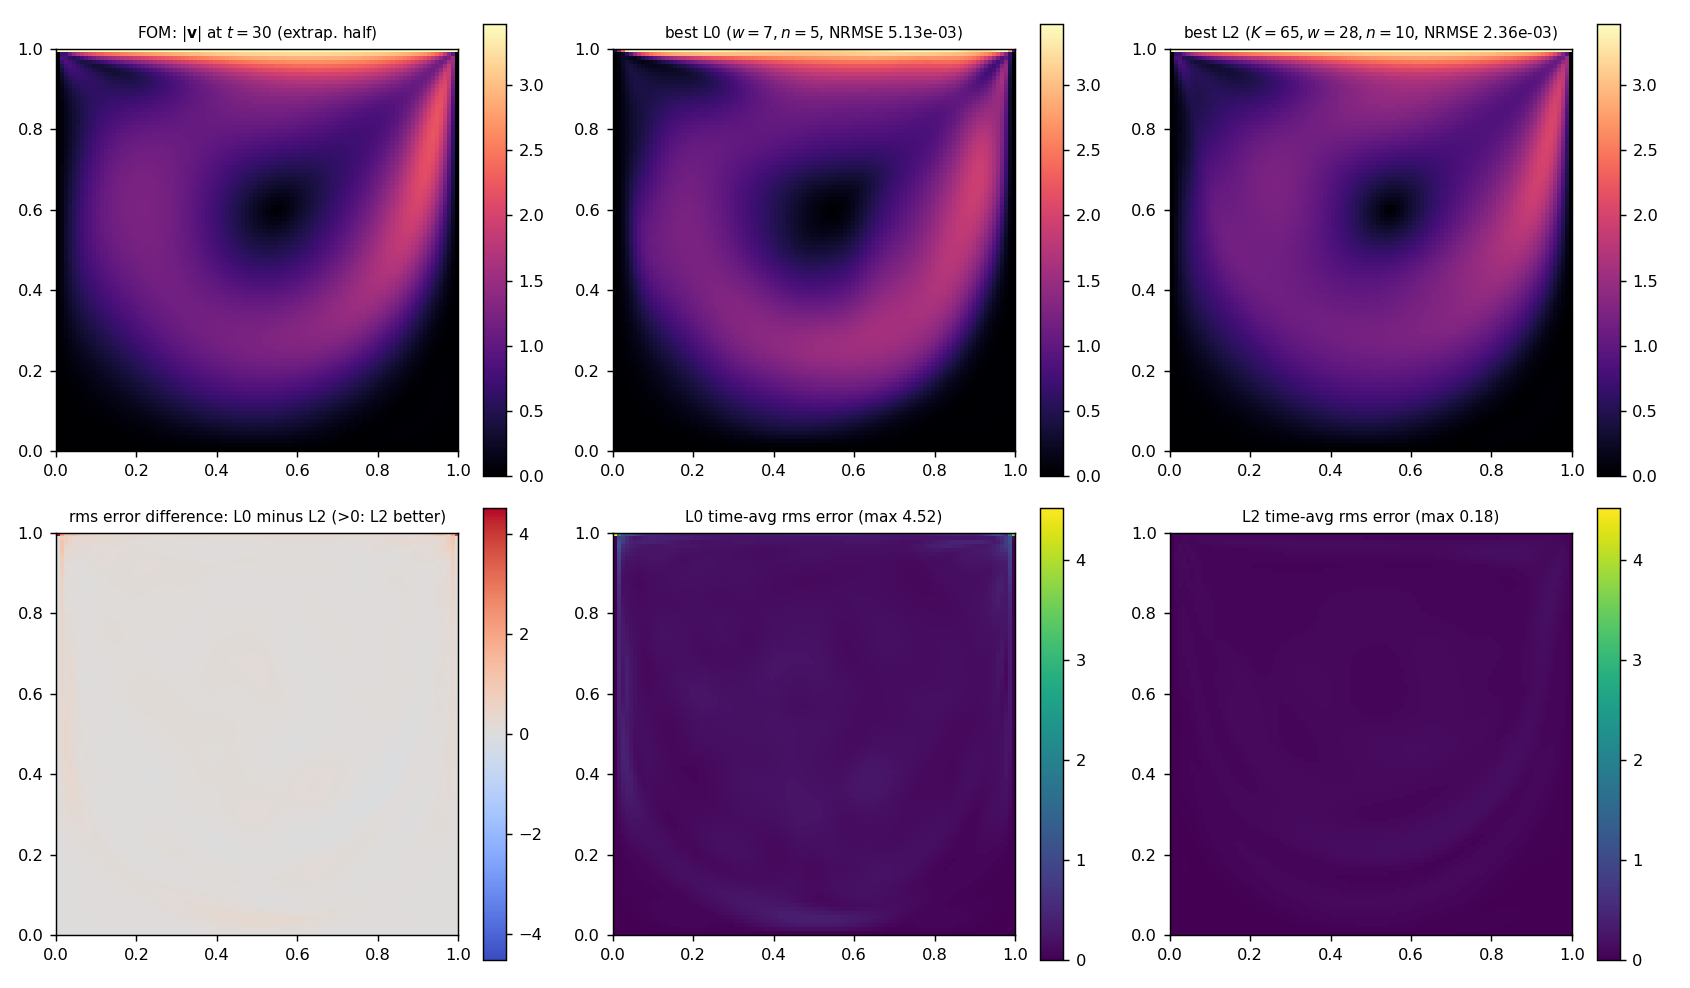
\includegraphics[width=0.90\textwidth,height=0.215\textheight,keepaspectratio]{fig8_B_fields_and_errors.png}
  \caption{Case B physical velocity fields and spatial error distribution at the $10{,}000$-iteration BFGS budget (test trajectory 0 at $t=30$, inside the time-extrapolation window $[20,40]$). \textbf{Top row:} velocity magnitude $\norm{\mathbf{v}}_2$ for the FOM ground truth (left), the best $\mathrm{L0}$ model ($w=7, L=2, n=5$, $\NRMSE = 5.86\cdot 10^{-3}$, centre), and the best $\mathrm{L2}$ model ($K=65, w=28, L=2, n=10$, $\NRMSE = 2.32\cdot 10^{-3}$, right). \textbf{Bottom row:} time-averaged pointwise rms error difference $\mathrm{err}_{\mathrm{L0}}(\mathbf{x}) - \mathrm{err}_{\mathrm{L2}}(\mathbf{x})$ (left, positive throughout the top-lid boundary layer and primary vortex core) and individual rms error maps of $\mathrm{L0}$ (centre) and $\mathrm{L2}$ (right) on a common colour scale.}
  \label{fig:rq2bis_fig8}
\end{figure}

\subsection{Case C Scalability Results: Steep \texorpdfstring{$\mathrm{L0}$}{L0} Capacity Law, Depth vs.\ Width, and Polynomial Overfitting of \texorpdfstring{$\mathrm{L2}$}{L2}}

Table~\ref{tab:rq2bis_caseC} reports all 21 configurations of Case~C at the $10{,}000$-iteration BFGS budget on CINECA Leonardo, and Figure~\ref{fig:rq2bis_fig9} compares the resulting space-time action-potential fields.

\begin{table}[!htbp]
\centering
\caption{Case C (\texttt{AP1D}): all 21 configurations at the $10{,}000$-iteration BFGS budget on CINECA Leonardo (median and $[\min,\max]$ over 3 seeds). Columns match Table~\ref{tab:rq2bis_caseB}, with Case~C's goal-oriented metrics: activation-time MAE (ms) and fraction of missed activations (\texttt{miss}).}
\label{tab:rq2bis_caseC}
\scriptsize
\setlength{\tabcolsep}{3.3pt}\resizebox{\textwidth}{!}{%

\begin{tabular}{@{}lrrrrrrrrrrrrrrlrr@{}}
\toprule
\textbf{Arm} & $K$ & $w$ & $L$ & $n$ & \textbf{st} & $P_{\mathrm{dyn}}$ & $P_{\mathrm{rec}}$ & $P_{\mathrm{tot}}$ & $\min\text{it}$ & $n_{\mathrm{fev}}$ & $s_{\mathrm{eval}}$[s] & $T_{\mathrm{PassT}}$[s] & $T_{\mathrm{PassA}}$[s] & \textbf{Valid} & \textbf{Test NRMSE $[\min,\max]$} & \textbf{MAE[ms]} & \textbf{miss} \\
\midrule
L0 & $0$ & $2$ & $1$ & $12$ & $0$ & $66$ & $1480$ & $1546$ & $10000$ & $10077$ & $0.266$ & $2680$ & $3700$ & $5.26\cdot 10^{-2}$ & $3.08\cdot 10^{-2}$ $[2.29, 7.51]\cdot 10^{-2}$ & $2.64$ & $0.001$ \\
L0 & $0$ & $4$ & $1$ & $12$ & $0$ & $120$ & $1480$ & $1600$ & $10000$ & $10042$ & $0.268$ & $2700$ & $3730$ & $9.58\cdot 10^{-3}$ & $1.15\cdot 10^{-2}$ $[8.99\cdot 10^{-3}, 1.56\cdot 10^{-2}]$ & $0.73$ & $0.000$ \\
L0 & $0$ & $8$ & $1$ & $3$ & $0$ & $75$ & $1327$ & $1402$ & $10000$ & $10035$ & $0.257$ & $2580$ & $3070$ & $1.40\cdot 10^{-2}$ & $2.22\cdot 10^{-2}$ $[1.06, 5.49]\cdot 10^{-2}$ & $1.09$ & $0.000$ \\
L0 & $0$ & $8$ & $1$ & $6$ & $0$ & $126$ & $1378$ & $1504$ & $10000$ & $10066$ & $0.268$ & $2700$ & $3460$ & $9.83\cdot 10^{-3}$ & $8.82\cdot 10^{-3}$ $[8.60, 9.31]\cdot 10^{-3}$ & $0.61$ & $0.000$ \\
L0 & $0$ & $8$ & $1$ & $12$ & $0$ & $228$ & $1480$ & $1708$ & $10000$ & $10071$ & $0.265$ & $2670$ & $4090$ & $9.00\cdot 10^{-3}$ & $1.01\cdot 10^{-2}$ $[7.88\cdot 10^{-3}, 1.14\cdot 10^{-2}]$ & $0.62$ & $0.000$ \\
L0 & $0$ & $8$ & $1$ & $24$ & $1$ & $432$ & $1684$ & $2116$ & $221$ & $10051$ & $0.303$ & $3040$ & $5210$ & $8.57\cdot 10^{-3}$ & $9.50\cdot 10^{-3}$ $[8.02\cdot 10^{-3}, 1.52\cdot 10^{-1}]$ & $0.56$ & $0.000$ \\
L0 & $0$ & $8$ & $2$ & $12$ & $0$ & $300$ & $1480$ & $1780$ & $10000$ & $10085$ & $0.279$ & $2810$ & $3990$ & $9.68\cdot 10^{-3}$ & $9.17\cdot 10^{-3}$ $[8.61\cdot 10^{-3}, 1.10\cdot 10^{-2}]$ & $0.59$ & $0.000$ \\
\textbf{L0} & $\mathbf{0}$ & $\mathbf{8}$ & $\mathbf{3}$ & $\mathbf{12}$ & $\mathbf{0}$ & $\mathbf{372}$ & $\mathbf{1480}$ & $\mathbf{1852}$ & $\mathbf{10000}$ & $\mathbf{10248}$ & $\mathbf{0.295}$ & $\mathbf{3020}$ & $\mathbf{4290}$ & $\mathbf{8.23\cdot 10^{-3}}$ & $\mathbf{7.83\cdot 10^{-3}}$ $[7.10, 8.04]\cdot 10^{-3}$ & $\mathbf{0.54}$ & $\mathbf{0.000}$ \\
L0 & $0$ & $16$ & $1$ & $12$ & $0$ & $444$ & $1480$ & $1924$ & $10000$ & $10059$ & $0.280$ & $2810$ & $4490$ & $8.62\cdot 10^{-3}$ & $9.65\cdot 10^{-3}$ $[9.05\cdot 10^{-3}, 1.10\cdot 10^{-2}]$ & $0.55$ & $0.001$ \\
L0 & $0$ & $32$ & $1$ & $12$ & $0$ & $876$ & $1480$ & $2356$ & $10000$ & $10051$ & $0.283$ & $2840$ & $5660$ & $8.65\cdot 10^{-3}$ & $8.57\cdot 10^{-3}$ $[8.22, 9.14]\cdot 10^{-3}$ & $0.56$ & $0.000$ \\
\midrule
L2 & $5$ & $8$ & $1$ & $12$ & $1$ & $228$ & $65$ & $293$ & $4368$ & $10221$ & $0.0489$ & $500$ & $589$ & $1.72\cdot 10^{-1}$ & $1.52\cdot 10^{-1}$ $[1.51, 1.56]\cdot 10^{-1}$ & $17.4$ & $0.006$ \\
L2 & $17$ & $8$ & $1$ & $12$ & $3$ & $228$ & $221$ & $449$ & $2833$ & $4999$ & $0.0511$ & $256$ & $342$ & $1.11\cdot 10^{-1}$ & $1.08\cdot 10^{-1}$ $[9.67\cdot 10^{-2}, 1.32\cdot 10^{-1}]$ & $5.41$ & $0.017$ \\
L2 & $33$ & $8$ & $1$ & $12$ & $1$ & $228$ & $429$ & $657$ & $3630$ & $10075$ & $0.0572$ & $576$ & $934$ & $1.07\cdot 10^{-1}$ & $1.02\cdot 10^{-1}$ $[1.00, 1.43]\cdot 10^{-1}$ & $4.91$ & $0.015$ \\
L2 & $65$ & $2$ & $1$ & $12$ & $3$ & $66$ & $845$ & $911$ & $1232$ & $1413$ & $0.0539$ & $76$ & $119$ & $2.79\cdot 10^{-1}$ & $2.43\cdot 10^{-1}$ $[2.43, 2.43]\cdot 10^{-1}$ & $14.1$ & $0.540$ \\
L2 & $65$ & $4$ & $1$ & $12$ & $3$ & $120$ & $845$ & $965$ & $1813$ & $2722$ & $0.0586$ & $160$ & $241$ & $1.63\cdot 10^{-1}$ & $1.59\cdot 10^{-1}$ $[1.52, 1.59]\cdot 10^{-1}$ & $10.5$ & $0.102$ \\
L2 & $65$ & $8$ & $1$ & $3$ & $0$ & $75$ & $260$ & $335$ & $10000$ & $10644$ & $0.0609$ & $648$ & $811$ & $1.95\cdot 10^{-1}$ & $1.70\cdot 10^{-1}$ $[1.65, 1.73]\cdot 10^{-1}$ & $21.4$ & $0.072$ \\
L2 & $65$ & $8$ & $1$ & $6$ & $0$ & $126$ & $455$ & $581$ & $10000$ & $10371$ & $0.0610$ & $632$ & $844$ & $1.19\cdot 10^{-1}$ & $1.05\cdot 10^{-1}$ $[1.03, 1.08]\cdot 10^{-1}$ & $6.85$ & $0.013$ \\
L2 & $65$ & $8$ & $1$ & $12$ & $1$ & $228$ & $845$ & $1073$ & $4149$ & $10051$ & $0.0596$ & $599$ & $1190$ & $1.06\cdot 10^{-1}$ & $1.02\cdot 10^{-1}$ $[9.38\cdot 10^{-2}, 1.66\cdot 10^{-1}]$ & $5.09$ & $0.014$ \\
L2 & $65$ & $8$ & $1$ & $24$ & $3$ & $432$ & $1625$ & $2057$ & $5277$ & $7561$ & $0.0752$ & $569$ & $2280$ & $1.05\cdot 10^{-1}$ & $9.49\cdot 10^{-2}$ $[9.29\cdot 10^{-2}, 2.03\cdot 10^{-1}]$ & $4.84$ & $0.018$ \\
\textbf{L2} & $\mathbf{65}$ & $\mathbf{16}$ & $\mathbf{1}$ & $\mathbf{12}$ & $\mathbf{1}$ & $\mathbf{444}$ & $\mathbf{845}$ & $\mathbf{1289}$ & $\mathbf{5409}$ & $\mathbf{10018}$ & $\mathbf{0.0666}$ & $\mathbf{667}$ & $\mathbf{1380}$ & $\mathbf{7.68\cdot 10^{-2}}$ & $\mathbf{1.05\cdot 10^{-1}}$ $[7.30\cdot 10^{-2}, 3.44\cdot 10^{-1}]$ & $\mathbf{2.26}$ & $\mathbf{0.005}$ \\
L2 & $65$ & $32$ & $1$ & $12$ & $1$ & $876$ & $845$ & $1721$ & $5968$ & $10099$ & $0.0863$ & $871$ & $2490$ & $1.01\cdot 10^{-1}$ & $1.22\cdot 10^{-1}$ $[8.07\cdot 10^{-2}, 1.45\cdot 10^{-1}]$ & $2.18$ & $0.005$ \\
\bottomrule
\end{tabular}
}
\end{table}

In Case~C, the roles of $\mathrm{L0}$ and $\mathrm{L2}$ reverse completely (Figure~\ref{fig:rq2bis_fig1} right):
\begin{enumerate}[leftmargin=2em]
  \item \textbf{Steep capacity scaling of $\mathrm{L0}$ up to the canonical knee $w^* = 8$:} In Case~C, $\NNdyn$ maps $14$ inputs ($12$ latent states plus $2$ stimulus channels) to $12$ latent derivatives through a single hidden layer of width $w$. At $w=2$ ($P_{\mathrm{dyn}} = 66$), the hidden layer is a rank-2 bottleneck (Proposition~\ref{prop:dyn_rank_bound}) that cannot even represent the 3-dimensional intrinsic wave manifold: median test NRMSE is $3.08\cdot 10^{-2}$ (activation MAE $2.64$~ms). Widening $w$ through $\{2, 4, 8, 16, 32\}$ reduces the test NRMSE monotonically:
  \begin{equation}
    3.08\cdot 10^{-2} \;\xrightarrow{w=4}\; 1.15\cdot 10^{-2} \;\xrightarrow{w=8}\; 1.01\cdot 10^{-2} \;\xrightarrow{w=16}\; 9.65\cdot 10^{-3} \;\xrightarrow{w=32}\; 8.57\cdot 10^{-3},
  \end{equation}
  following a steep power law with $E_\infty = 8.57\cdot 10^{-3}$ and $\alpha = 3.220$ (95\% CI $[1.882, 4.768]$), with the validation-selected knee located at the canonical width **$w^* = 8$** ($P_{\mathrm{dyn}} = 228$).
  \item \textbf{Dynamics depth beats dynamics width in Case C $\mathrm{L0}$:} Holding the width at $w^* = 8$ and increasing the number of hidden layers from $L=1$ ($P_{\mathrm{dyn}} = 228$, $\NRMSE = 1.01\cdot 10^{-2}$) to $L=2$ ($P_{\mathrm{dyn}} = 300$, $\NRMSE = 9.17\cdot 10^{-3}$) and $L=3$ ($P_{\mathrm{dyn}} = 372$, $P_{\mathrm{total}} = 1852$) yields the \textbf{lowest validation ($8.23\cdot 10^{-3}$) and test ($\mathbf{7.83\cdot 10^{-3}}$, range $[7.10, 8.04]\cdot 10^{-3}$) NRMSE of the entire Case~C campaign}, achieving sub-millisecond front arrival accuracy ($\mathbf{0.54}$~\textbf{ms MAE}, $0.0\%$ missed activations) and outperforming the widest single-layer network $w=32, L=1$ ($8.57\cdot 10^{-3}$ at $P_{\mathrm{dyn}} = 876$) with \textbf{$2.35\times$ fewer dynamics parameters}! Composing three nonlinear hidden layers allows $\NNdyn$ to represent the stiff fast--slow reaction kinetics of the Aliev--Panfilov equations far more compactly than a single wide layer.
  \item \textbf{Why $\mathrm{L2}$ stalls and overfits in Case C:} Even when expanded to $K = 65$ Legendre modes and $n = 24$ latent states, $\mathrm{L2}$ never drops below a median test NRMSE of $9.49\cdot 10^{-2}$ ($12.1\times$ worse than the best $\mathrm{L0}$). Moreover, at $K=65, n=12$, widening $\NNdyn$ to $w=16$ and $w=32$ causes the test NRMSE to reach its minimum around iteration $1{,}000$ ($7.18\cdot 10^{-2}$ at $w=16$, $6.26\cdot 10^{-2}$ at $w=32$) and then \textbf{degrade between iterations $1{,}000$ and $10{,}000$} back up to $1.05\cdot 10^{-1}$ and $1.22\cdot 10^{-1}$! The mechanism is classical polynomial aliasing: during training, the loss is evaluated on only $N_x = 20$ random spatial points per time step, whereas the reconstructor synthesises $K = 65$ Legendre polynomials up to degree $64$. Once $\NNdyn$ is wide enough ($w \ge 16$), thousands of BFGS iterations drive the 20-point training loss down by fitting high-degree polynomial oscillations between the 20 sampled points, which explode when evaluated on the full 101-point test grid (Figure~\ref{fig:rq2bis_fig9}).
\end{enumerate}

\begin{figure}[!htbp]
  \centering
  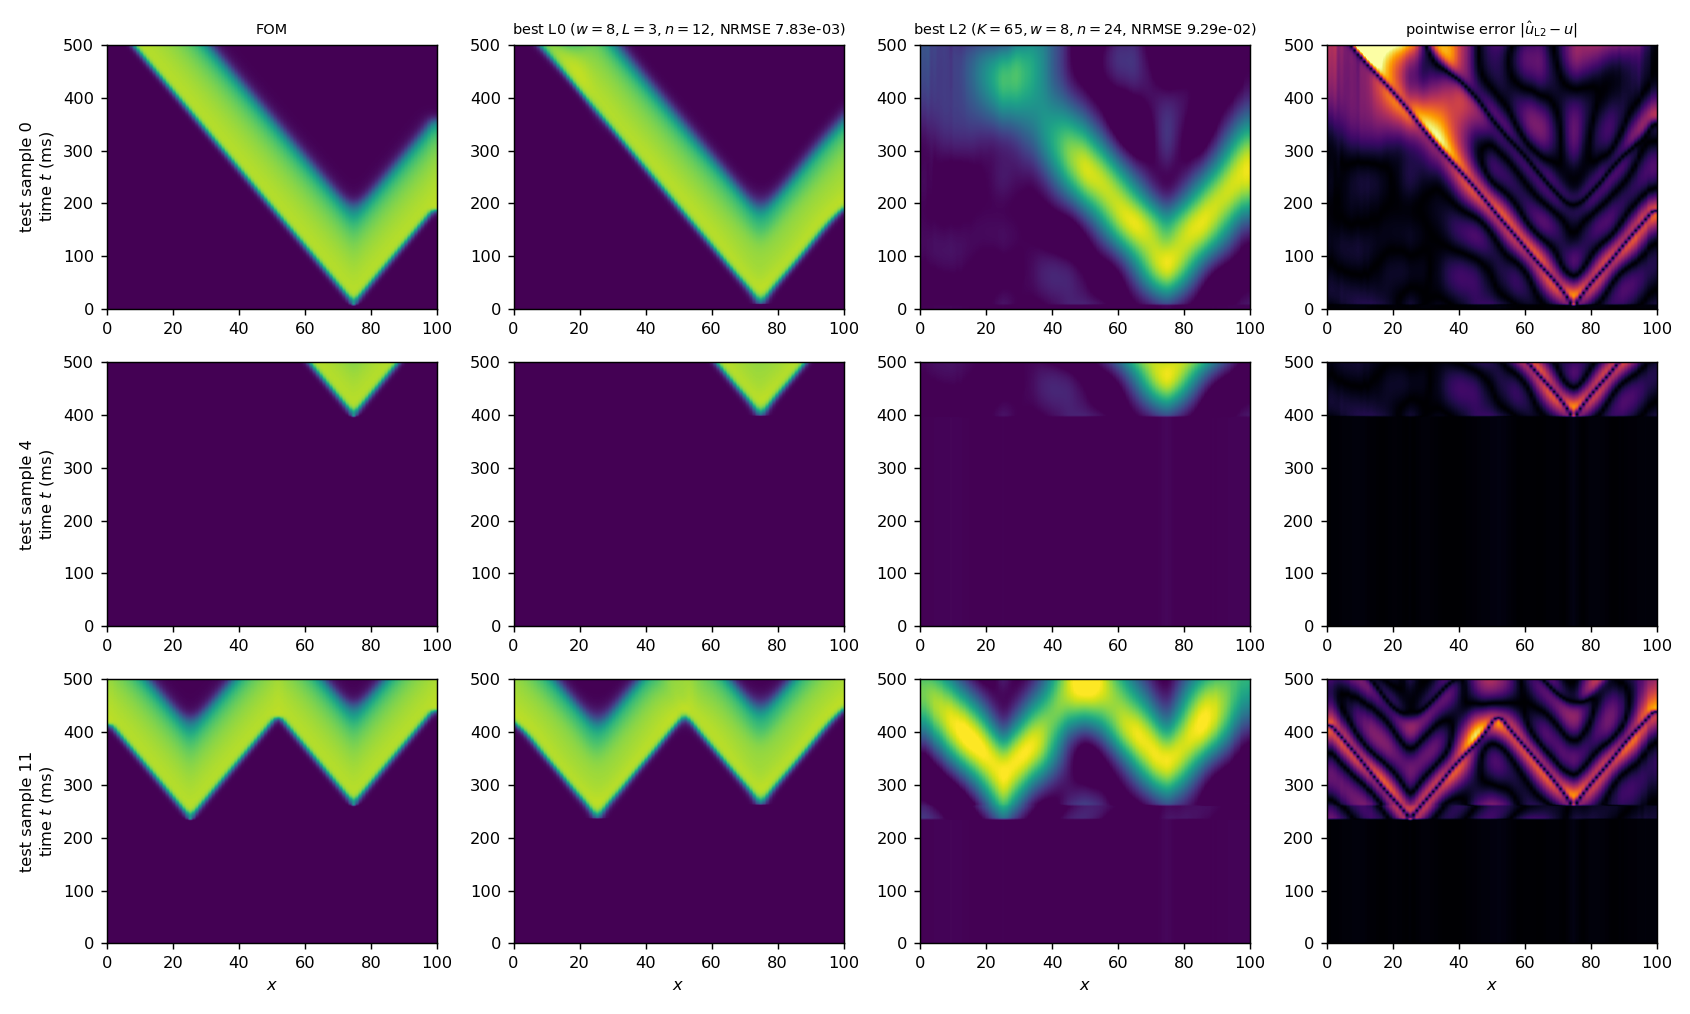
\includegraphics[width=0.90\textwidth,height=0.215\textheight,keepaspectratio]{fig9_C_fronts_comparison.png}
  \caption{Case C space-time transmembrane potential $u(x,t)$ on three test trajectories (rows: test samples 0, 4, and 11) at the $10{,}000$-iteration BFGS budget. \textbf{Columns:} FOM ground truth; best $\mathrm{L0}$ configuration ($w=8, L=3, n=12$, seed 0 $\NRMSE = 7.10\cdot 10^{-3}$); best $\mathrm{L2}$ configuration on test ($K=65, w=8, L=1, n=24$, seed 0 $\NRMSE = 9.29\cdot 10^{-2}$); and pointwise absolute error $|\hat{u}_{\mathrm{L2}}(x,t) - u(x,t)|$, demonstrating how linear polynomial synthesis concentrates error along the moving depolarisation wave fronts and generates global Gibbs oscillations.}
  \label{fig:rq2bis_fig9}
\end{figure}

\subsection{The Iteration Surface \texorpdfstring{$\NRMSE(w, \text{iterations})$}{NRMSE(w, iterations)} and 1,000 vs.\ 10,000 Iterations}

Figures~\ref{fig:rq2bis_fig2}, \ref{fig:rq2bis_fig4}, and~\ref{fig:rq2bis_fig6} and Table~\ref{tab:rq2bis_checkpoints} present the evolution of the test NRMSE across the nine BFGS checkpoints~\eqref{eq:checkpoints}, alongside the direct comparison between the $1{,}000$-iteration laptop pilot and the $10{,}000$-iteration CINECA Leonardo cluster sweep.

\begin{figure}[!htbp]
  \centering
  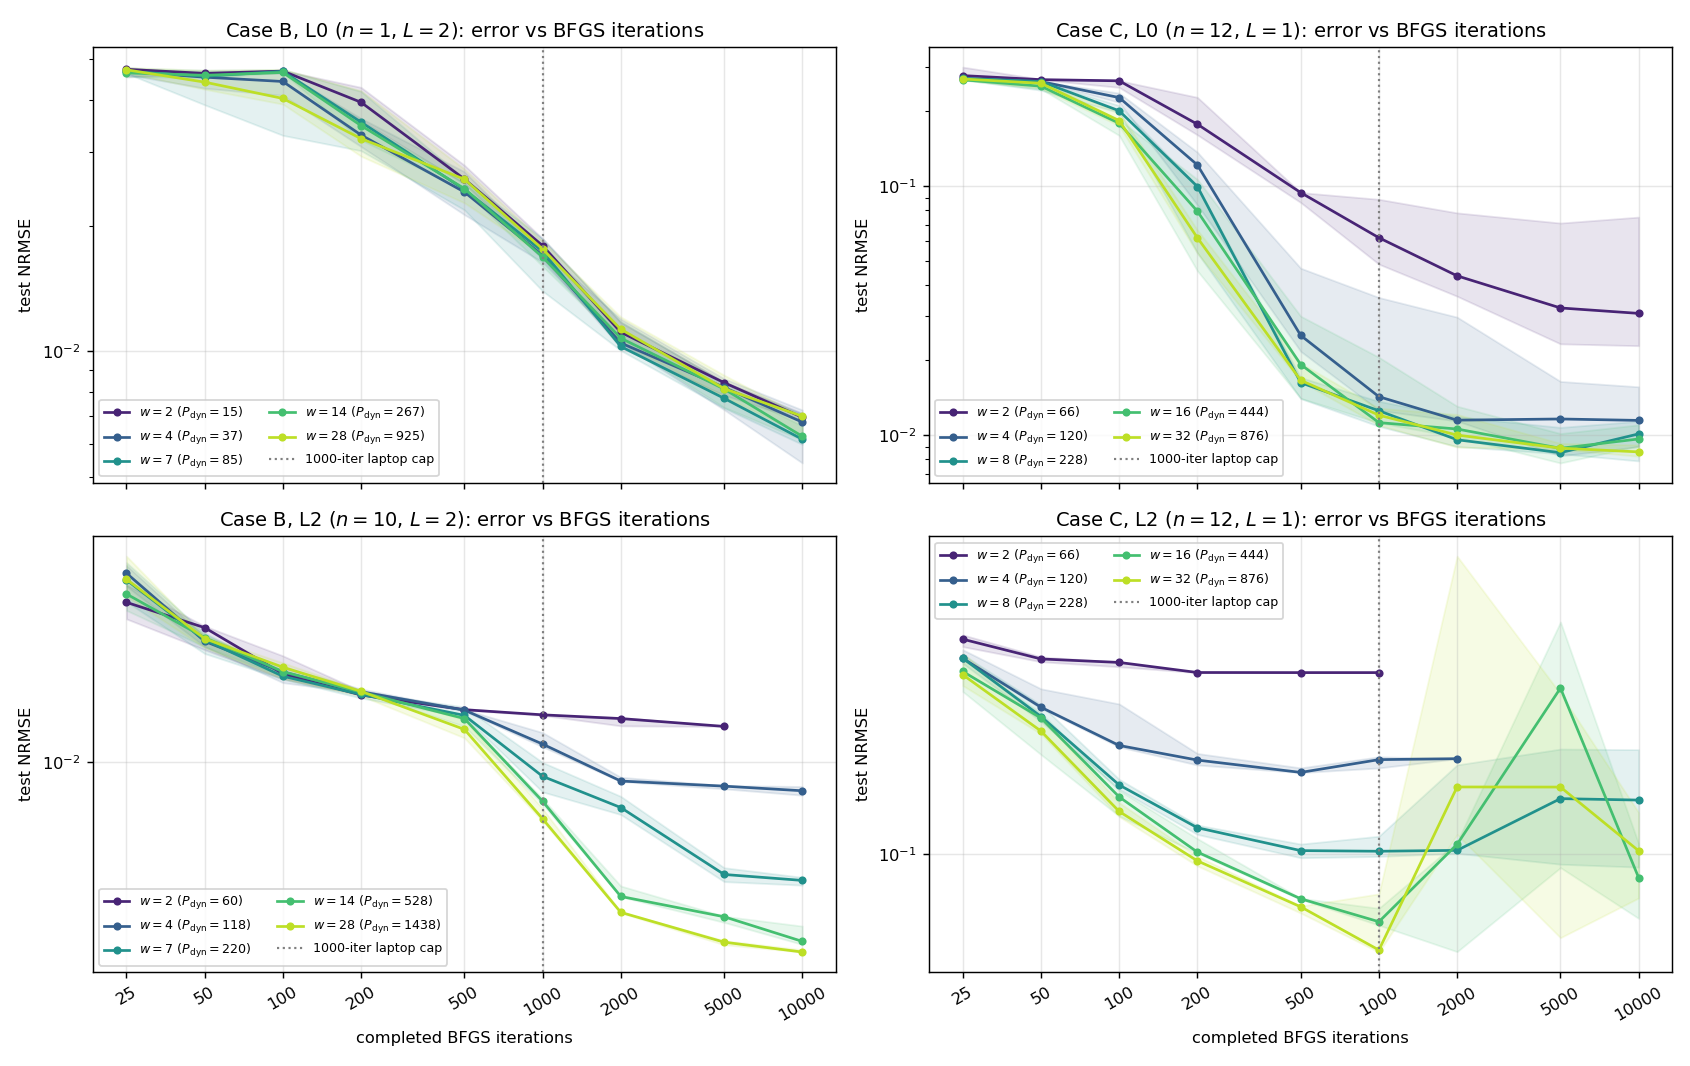
\includegraphics[width=0.90\textwidth,height=0.215\textheight,keepaspectratio]{fig2_iteration_surface.png}
  \caption{Stage~3 quasi-Newton iteration surface: test NRMSE (median and min--max band of 3 seeds) as a function of completed BFGS iterations $k \in \{25, 50, 100, 200, 500, 1000, 2000, 5000, 10000\}$ across dynamics hidden widths $w$, for Case~B (\textbf{left}) and Case~C (\textbf{right}), in the nonlinear arm $\mathrm{L0}$ (\textbf{top}) and linear arm $\mathrm{L2}$ (\textbf{bottom}). The vertical dotted line indicates the $1{,}000$-iteration pilot cap.}
  \label{fig:rq2bis_fig2}
\end{figure}

\begin{figure}[!htbp]
  \centering
  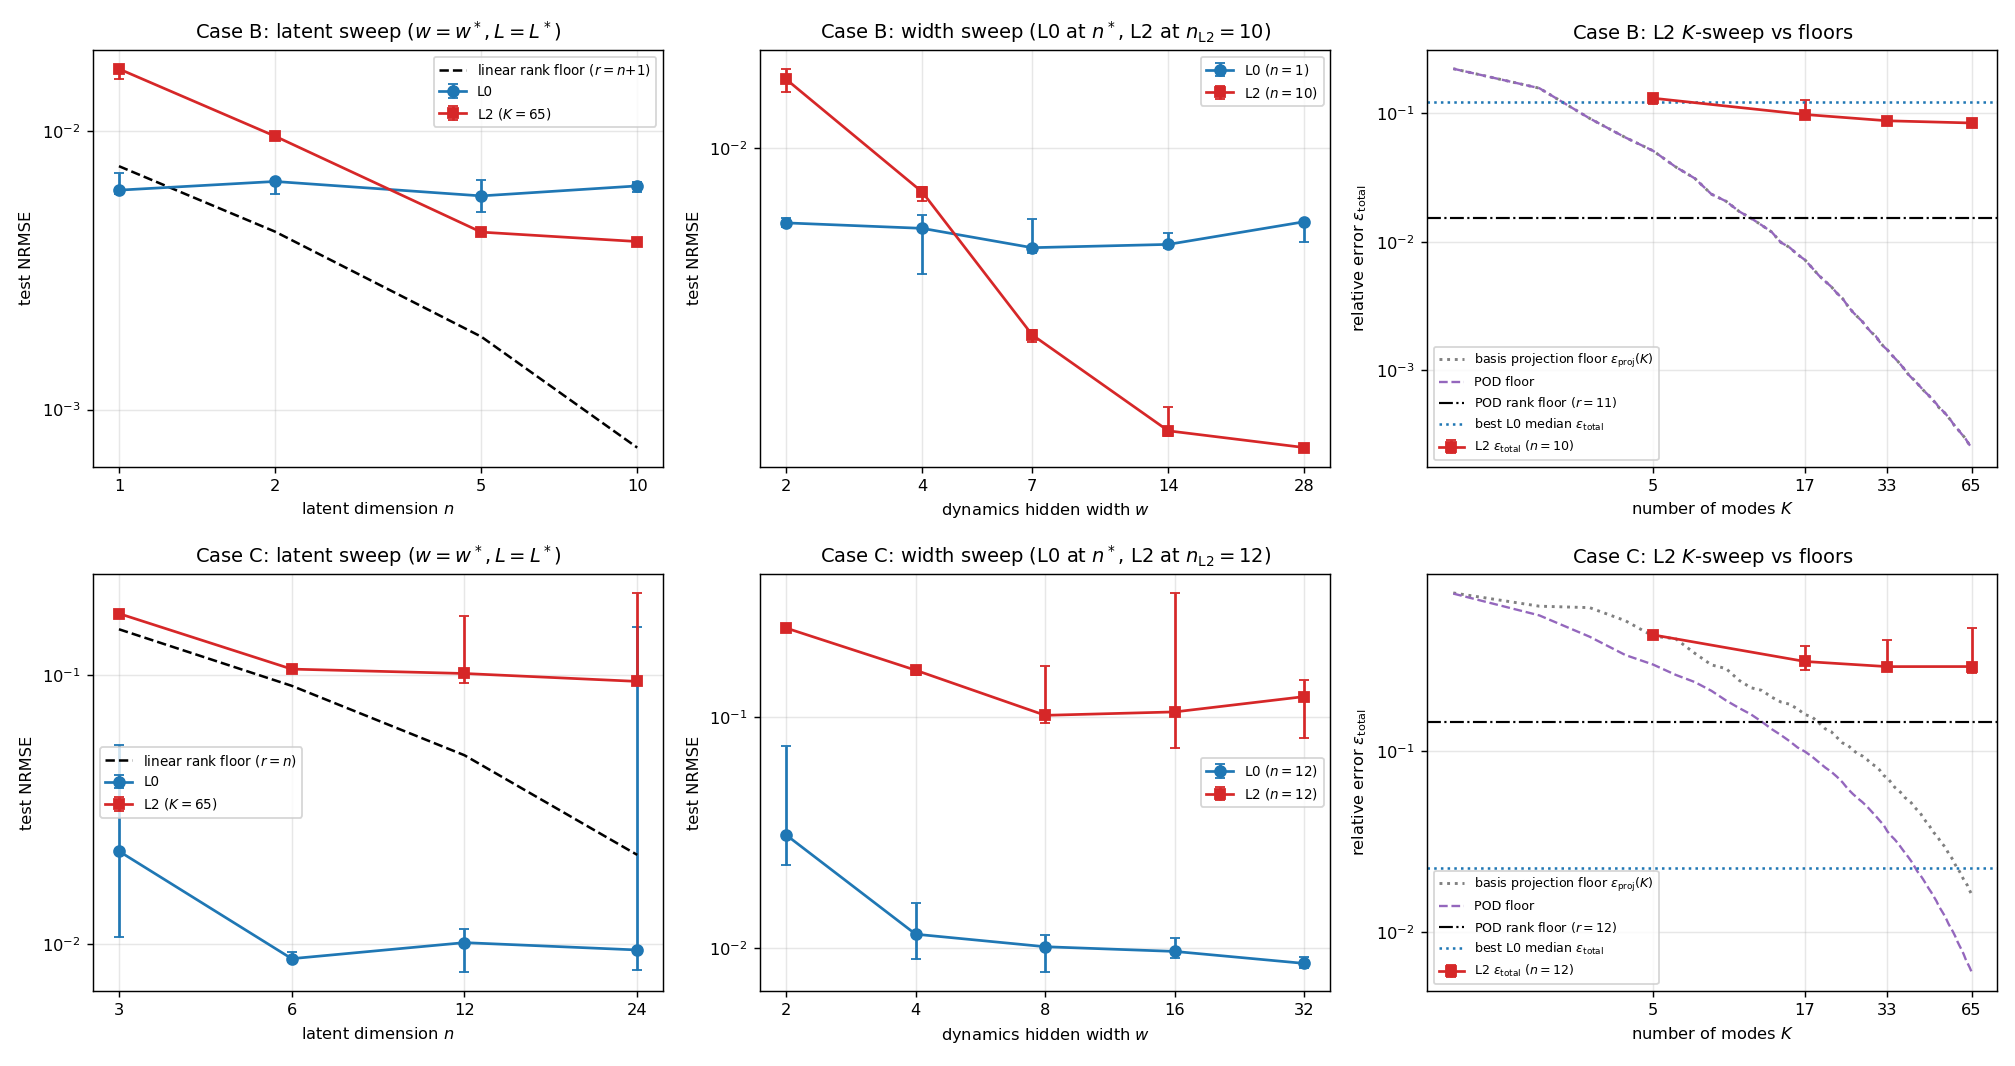
\includegraphics[width=0.90\textwidth,height=0.215\textheight,keepaspectratio]{fig4_linear_arm_sweeps.png}
  \caption{Stage~7 linear reconstructor arm ($\mathrm{L2}$, red squares) versus nonlinear reconstructor arm ($\mathrm{L0}$, blue circles) at $10{,}000$ BFGS iterations in Case~B (\textbf{top row}) and Case~C (\textbf{bottom row}): test NRMSE against latent dimension $n$ with the POD rank floor (left), against dynamics hidden width $w$ (centre), and relative test error $\varepsilon_{\mathrm{total}}$ against basis size $K$ compared with $\varepsilon_{\mathrm{proj}}(K)$ and the POD rank floor (right).}
  \label{fig:rq2bis_fig4}
\end{figure}

\begin{figure}[!htbp]
  \centering
  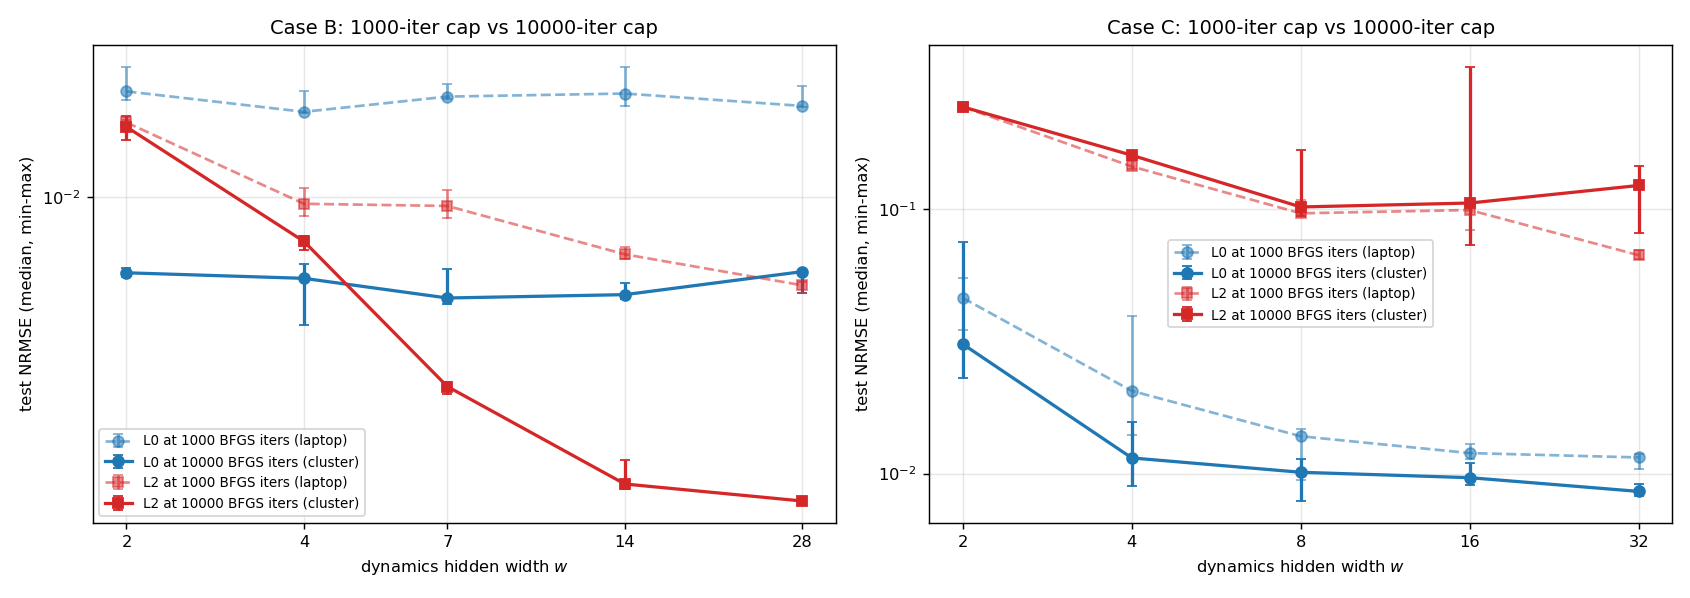
\includegraphics[width=0.90\textwidth,height=0.215\textheight,keepaspectratio]{fig6_budget_1000_vs_10000.png}
  \caption{Impact of the tenfold increase in quasi-Newton budget from the $1{,}000$-iteration laptop sweep (dashed curves) to the $10{,}000$-iteration CINECA Leonardo cluster sweep (solid curves) across the dynamics width sweeps of Case~B (\textbf{left}) and Case~C (\textbf{right}).}
  \label{fig:rq2bis_fig6}
\end{figure}

\begin{table}[!htbp]
\centering
\caption{Stage~3 checkpoint evolution: median test NRMSE across completed BFGS iterations $k \in \{50, 200, 500, 1000, 2000, 5000, 10000\}$ on the dynamics width sweeps of Cases~B and~C, together with the relative error reduction between iteration $1{,}000$ and iteration $10{,}000$.}
\label{tab:rq2bis_checkpoints}
\footnotesize\resizebox{\textwidth}{!}{%

\begin{tabular}{@{}llrrrrrrrrr@{}}
\toprule
\textbf{Case \& Arm} & $w$ & $P_{\mathrm{dyn}}$ & \textbf{iter 50} & \textbf{iter 200} & \textbf{iter 500} & \textbf{iter 1000} & \textbf{iter 2000} & \textbf{iter 5000} & \textbf{iter 10000} & \textbf{Drop $1\text{k}\to 10\text{k}$} \\
\midrule
\textbf{B, L0} ($n{=}1, L{=}2$)
 & $2$  & $15$  & $4.63\cdot 10^{-2}$ & $3.95\cdot 10^{-2}$ & $2.58\cdot 10^{-2}$ & $1.79\cdot 10^{-2}$ & $1.11\cdot 10^{-2}$ & $8.40\cdot 10^{-3}$ & $6.94\cdot 10^{-3}$ & $\mathbf{+61.2\%}$ \\
 & $4$  & $37$  & $4.54\cdot 10^{-2}$ & $3.30\cdot 10^{-2}$ & $2.41\cdot 10^{-2}$ & $1.70\cdot 10^{-2}$ & $1.05\cdot 10^{-2}$ & $8.19\cdot 10^{-3}$ & $6.76\cdot 10^{-3}$ & $\mathbf{+60.2\%}$ \\
 & $7$  & $85$  & $4.56\cdot 10^{-2}$ & $3.54\cdot 10^{-2}$ & $2.44\cdot 10^{-2}$ & $1.73\cdot 10^{-2}$ & $1.03\cdot 10^{-2}$ & $7.71\cdot 10^{-3}$ & $6.15\cdot 10^{-3}$ & $\mathbf{+64.5\%}$ \\
 & $14$ & $267$ & $4.58\cdot 10^{-2}$ & $3.47\cdot 10^{-2}$ & $2.45\cdot 10^{-2}$ & $1.68\cdot 10^{-2}$ & $1.07\cdot 10^{-2}$ & $8.11\cdot 10^{-3}$ & $6.25\cdot 10^{-3}$ & $\mathbf{+62.8\%}$ \\
 & $28$ & $925$ & $4.41\cdot 10^{-2}$ & $3.23\cdot 10^{-2}$ & $2.58\cdot 10^{-2}$ & $1.76\cdot 10^{-2}$ & $1.13\cdot 10^{-2}$ & $8.13\cdot 10^{-3}$ & $6.98\cdot 10^{-3}$ & $\mathbf{+60.3\%}$ \\
\midrule
\textbf{B, L2} ($n{=}10, K{=}65$)
 & $2$  & $60$   & $2.80\cdot 10^{-2}$ & $1.67\cdot 10^{-2}$ & $1.49\cdot 10^{-2}$ & $1.43\cdot 10^{-2}$ & $1.39\cdot 10^{-2}$ & $1.31\cdot 10^{-2}$ & $1.40\cdot 10^{-2}$ (st) & $+2.1\%$ \\
 & $4$  & $118$  & $2.52\cdot 10^{-2}$ & $1.71\cdot 10^{-2}$ & $1.49\cdot 10^{-2}$ & $1.15\cdot 10^{-2}$ & $8.62\cdot 10^{-3}$ & $8.29\cdot 10^{-3}$ & $8.07\cdot 10^{-3}$ & $\mathbf{+30.1\%}$ \\
 & $7$  & $220$  & $2.55\cdot 10^{-2}$ & $1.68\cdot 10^{-2}$ & $1.43\cdot 10^{-2}$ & $8.94\cdot 10^{-3}$ & $7.03\cdot 10^{-3}$ & $4.21\cdot 10^{-3}$ & $4.02\cdot 10^{-3}$ & $\mathbf{+55.0\%}$ \\
 & $14$ & $528$  & $2.59\cdot 10^{-2}$ & $1.71\cdot 10^{-2}$ & $1.39\cdot 10^{-2}$ & $7.38\cdot 10^{-3}$ & $3.55\cdot 10^{-3}$ & $3.04\cdot 10^{-3}$ & $2.52\cdot 10^{-3}$ & $\mathbf{+65.9\%}$ \\
 & $28$ & $1438$ & $2.57\cdot 10^{-2}$ & $1.72\cdot 10^{-2}$ & $1.28\cdot 10^{-2}$ & $6.45\cdot 10^{-3}$ & $3.15\cdot 10^{-3}$ & $2.50\cdot 10^{-3}$ & $2.32\cdot 10^{-3}$ & $\mathbf{+64.1\%}$ \\
\midrule
\textbf{C, L0} ($n{=}12, L{=}1$)
 & $2$  & $66$  & $2.68\cdot 10^{-1}$ & $1.77\cdot 10^{-1}$ & $9.42\cdot 10^{-2}$ & $6.21\cdot 10^{-2}$ & $4.36\cdot 10^{-2}$ & $3.24\cdot 10^{-2}$ & $3.08\cdot 10^{-2}$ & $\mathbf{+50.3\%}$ \\
 & $4$  & $120$ & $2.63\cdot 10^{-1}$ & $1.22\cdot 10^{-1}$ & $2.52\cdot 10^{-2}$ & $1.43\cdot 10^{-2}$ & $1.15\cdot 10^{-2}$ & $1.16\cdot 10^{-2}$ & $1.15\cdot 10^{-2}$ & $\mathbf{+19.7\%}$ \\
 & $8$  & $228$ & $2.63\cdot 10^{-1}$ & $9.97\cdot 10^{-2}$ & $1.63\cdot 10^{-2}$ & $1.25\cdot 10^{-2}$ & $9.58\cdot 10^{-3}$ & $8.50\cdot 10^{-3}$ & $1.01\cdot 10^{-2}$ & $\mathbf{+19.3\%}$ \\
 & $16$ & $444$ & $2.52\cdot 10^{-1}$ & $7.93\cdot 10^{-2}$ & $1.92\cdot 10^{-2}$ & $1.12\cdot 10^{-2}$ & $1.06\cdot 10^{-2}$ & $8.85\cdot 10^{-3}$ & $9.65\cdot 10^{-3}$ & $\mathbf{+14.0\%}$ \\
 & $32$ & $876$ & $2.59\cdot 10^{-1}$ & $6.21\cdot 10^{-2}$ & $1.66\cdot 10^{-2}$ & $1.20\cdot 10^{-2}$ & $1.00\cdot 10^{-2}$ & $8.86\cdot 10^{-3}$ & $8.57\cdot 10^{-3}$ & $\mathbf{+28.8\%}$ \\
\midrule
\textbf{C, L2} ($n{=}12, K{=}65$)
 & $2$  & $66$  & $2.59\cdot 10^{-1}$ & $2.43\cdot 10^{-1}$ & $2.43\cdot 10^{-1}$ & $2.43\cdot 10^{-1}$ & -- & -- & $2.43\cdot 10^{-1}$ (st) & $0.0\%$ \\
 & $4$  & $120$ & $2.05\cdot 10^{-1}$ & $1.58\cdot 10^{-1}$ & $1.49\cdot 10^{-1}$ & $1.59\cdot 10^{-1}$ & $1.59\cdot 10^{-1}$ & -- & $1.59\cdot 10^{-1}$ (st) & $-0.4\%$ \\
 & $8$  & $228$ & $1.96\cdot 10^{-1}$ & $1.14\cdot 10^{-1}$ & $1.02\cdot 10^{-1}$ & $1.01\cdot 10^{-1}$ & $1.02\cdot 10^{-1}$ & $1.31\cdot 10^{-1}$ & $1.02\cdot 10^{-1}$ & $-0.3\%$ \\
 & $16$ & $444$ & $1.94\cdot 10^{-1}$ & $1.01\cdot 10^{-1}$ & $8.04\cdot 10^{-2}$ & $\mathbf{7.18\cdot 10^{-2}}$ & $1.05\cdot 10^{-1}$ & $2.25\cdot 10^{-1}$ & $1.05\cdot 10^{-1}$ & $\mathbf{-46.3\%}$ (overfit) \\
 & $32$ & $876$ & $1.82\cdot 10^{-1}$ & $9.67\cdot 10^{-2}$ & $7.73\cdot 10^{-2}$ & $\mathbf{6.26\cdot 10^{-2}}$ & $1.39\cdot 10^{-1}$ & $1.39\cdot 10^{-1}$ & $1.22\cdot 10^{-1}$ & $\mathbf{-95.8\%}$ (overfit) \\
\bottomrule
\end{tabular}
}
\end{table}

Table~\ref{tab:rq2bis_checkpoints} and Figure~\ref{fig:rq2bis_fig2} demonstrate why stopping quasi-Newton optimization at $500$ or $1{,}000$ iterations distorts architectural comparisons:
\begin{itemize}[leftmargin=2em]
  \item Between iteration $1{,}000$ and iteration $10{,}000$, every Case~B $\mathrm{L0}$ configuration drops by a further \textbf{$60.2\%$ to $64.5\%$} (from $\sim 1.7\cdot 10^{-2}$ down to $6.15$--$6.98\cdot 10^{-3}$), and every wide Case~B $\mathrm{L2}$ configuration ($w \in \{7, 14, 28\}$) drops by a further \textbf{$55.0\%$ to $65.9\%$} (from $8.94, 7.38, 6.45\cdot 10^{-3}$ down to $4.02, 2.52, 2.32\cdot 10^{-3}$). At iteration $500$, the five widths of Case~B $\mathrm{L2}$ were still bunched tightly between $1.28\cdot 10^{-2}$ and $1.49\cdot 10^{-2}$; only between iterations $1{,}000$ and $10{,}000$ does the $6\times$ capacity separation between $w=2$ ($1.40\cdot 10^{-2}$) and $w=28$ ($2.32\cdot 10^{-3}$) fully emerge!
  \item In Case~C $\mathrm{L0}$, at iteration $500$ the width curve is non-monotone ($[0.0942, 0.0252, 0.0163, 0.0192, 0.0166]$), because the larger networks ($w=16, 32$) have more parameters ($P_{\mathrm{total}} = 1924, 2356$) and require more quasi-Newton rank-2 updates to build an accurate inverse-Hessian approximation (Hypothesis~H3). By iteration $10{,}000$, all five widths have converged and the curve becomes strictly monotone decreasing ($[0.0308, 0.0115, 0.0101, 0.00965, 0.00857]$), falsifying Hypothesis~H3 at $10{,}000$ iterations in Case~C $\mathrm{L0}$ while still supporting it in Case~B $\mathrm{L0}$ (where the largest network $w=28, P_{\mathrm{total}} = 2895$ remains slightly above $w=7$, $6.98\cdot 10^{-3}$ vs.\ $6.15\cdot 10^{-3}$).
\end{itemize}

\subsection{Empirical Verification of the Dynamics Bottleneck Rank Bound (\texorpdfstring{$\mathrm{H4}$}{H4})}

To test Proposition~\ref{prop:dyn_rank_bound} directly on the trained models of \texttt{RQ2-bis}, we rebuilt all stored $\mathrm{L0}$ and $\mathrm{L2}$ networks in pure NumPy from \texttt{results/weights/}, rolled out the test-set latent trajectories $S_{\mathrm{traj}} \in \R^{(S_{\mathrm{test}} N_t) \times n}$, computed the exact analytical state-transition Jacobians $J(\mathbf{s}^{(s)}(t_i), \mathbf{u}^{(s)}(t_i)) = \partial\dot{\mathbf{s}}/\partial\mathbf{s} \in \R^{n \times n}$, and evaluated the numerical rank (number of singular values $\sigma_k > 10^{-3}\sigma_1$) of both matrices across all three seeds. Figure~\ref{fig:rq2bis_fig7} and Table~\ref{tab:rq2bis_ranks} report the results.

\begin{figure}[!htbp]
  \centering
  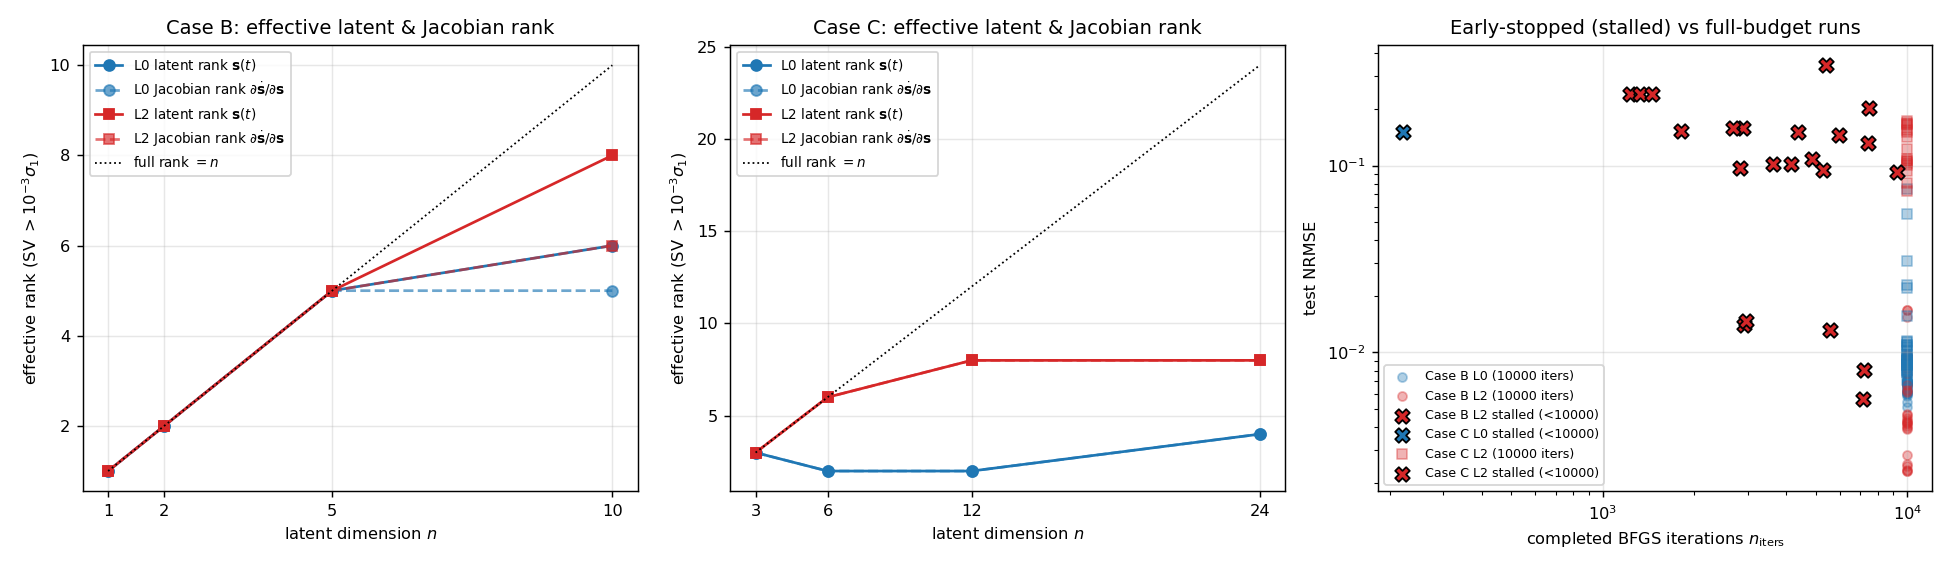
\includegraphics[width=0.90\textwidth,height=0.215\textheight,keepaspectratio]{fig7_ranks_and_stalls.png}
  \caption{\textbf{Left and centre:} empirical SVD rank (number of singular values $> 10^{-3}\sigma_1$, median over 3 seeds) of the test latent trajectories $\mathbf{s}(t)$ (solid lines) and of the state-transition Jacobians $\partial\dot{\mathbf{s}}/\partial\mathbf{s}$ (dashed lines) as a function of latent dimension $n$ at canonical dynamics hidden width ($w^*=7$ in Case~B, $w^*=8$ in Case~C). Both hit the exact algebraic ceiling of Proposition~\ref{prop:dyn_rank_bound}. \textbf{Right:} final test NRMSE versus completed BFGS iterations $n_{\mathrm{iters}}$ across all 126 cluster runs, highlighting the 23 early-stopped (\texttt{stalled}) runs.}
  \label{fig:rq2bis_fig7}
\end{figure}

\begin{table}[!htbp]
\centering
\caption{Empirical SVD rank (singular values $> 10^{-3}\sigma_1$ across seeds $[s_0, s_1, s_2]$) and smallest-to-largest singular-value ratio $\sigma_n/\sigma_1$ of the test latent trajectories $S_{\mathrm{traj}}$ and dynamics Jacobians $\partial\dot{\mathbf{s}}/\partial\mathbf{s}$, compared against the theoretical structural ceiling of Proposition~\ref{prop:dyn_rank_bound}.}
\label{tab:rq2bis_ranks}
\footnotesize\resizebox{\textwidth}{!}{%

\begin{tabular}{@{}llrrcllrr@{}}
\toprule
\textbf{Case} & \textbf{Arm} & \textbf{Width $w$} & \textbf{Latent $n$} & \textbf{Prop.~\ref{prop:dyn_rank_bound} Ceiling} & \textbf{Traj.\ Rank $[s_0,s_1,s_2]$} & \textbf{Jac.\ Rank $[s_0,s_1,s_2]$} & \textbf{Med.\ $\frac{\sigma_n}{\sigma_1}(\mathbf{s})$} & \textbf{Med.\ $\frac{\sigma_n}{\sigma_1}(J)$} \\
\midrule
\textbf{B} & L0 & $7$ ($w^*$) & $1$ & $1$ & $[1, 1, 1]$ & $[1, 1, 1]$ & $1.00$ & $1.00$ \\
 & L0 & $7$ ($w^*$) & $2$ & $2$ & $[2, 2, 2]$ & $[2, 2, 2]$ & $1.33\cdot 10^{-1}$ & $2.25\cdot 10^{-1}$ \\
 & L0 & $7$ ($w^*$) & $5$ & $5$ & $[5, 5, 5]$ & $[4, 5, 5]$ & $4.49\cdot 10^{-3}$ & $1.63\cdot 10^{-2}$ \\
 & L0 & $7$ ($w^*$) & $10$ & $\mathbf{8}$ ($w^*+1$) & $\mathbf{[6, 7, 6]}$ & $\mathbf{[5, 5, 6]}$ & $\mathbf{9.23\cdot 10^{-17}}$ & $\mathbf{5.25\cdot 10^{-18}}$ \\
 & L2 & $7$ ($w^*$) & $1$ & $1$ & $[1, 1, 1]$ & $[1, 1, 1]$ & $1.00$ & $1.00$ \\
 & L2 & $7$ ($w^*$) & $2$ & $2$ & $[2, 2, 2]$ & $[2, 2, 2]$ & $4.84\cdot 10^{-1}$ & $1.83\cdot 10^{-1}$ \\
 & L2 & $7$ ($w^*$) & $5$ & $5$ & $[5, 5, 5]$ & $[5, 5, 5]$ & $2.19\cdot 10^{-2}$ & $3.67\cdot 10^{-2}$ \\
 & L2 & $7$ ($w^*$) & $10$ & $\mathbf{8}$ ($w^*+1$) & $\mathbf{[8, 7, 8]}$ & $\mathbf{[5, 6, 6]}$ & $\mathbf{1.21\cdot 10^{-16}}$ & $\mathbf{5.83\cdot 10^{-18}}$ \\
 & \textbf{L2} & $\mathbf{28}$ ($4w^*$) & $\mathbf{10}$ & $\mathbf{10}$ & $\mathbf{[10, 10, 10]}$ & $\mathbf{[10, 10, 10]}$ & $> 10^{-3}$ & $> 10^{-3}$ \\
\midrule
\textbf{C} & L0 & $8$ ($w^*$) & $3$ & $3$ & $[3, 2, 3]$ & $[3, 2, 3]$ & $3.07\cdot 10^{-2}$ & $1.29\cdot 10^{-1}$ \\
 & L0 & $8$ ($w^*$) & $6$ & $6$ & $\mathbf{[2, 2, 2]}$ & $\mathbf{[2, 2, 2]}$ & $6.16\cdot 10^{-7}$ & $1.00\cdot 10^{-6}$ \\
 & L0 & $8$ ($w^*$) & $12$ & $\mathbf{8}$ ($w^*$) & $\mathbf{[2, 3, 2]}$ & $\mathbf{[2, 4, 2]}$ & $\mathbf{6.46\cdot 10^{-17}}$ & $\mathbf{2.18\cdot 10^{-18}}$ \\
 & L0 & $8$ ($w^*$) & $24$ & $\mathbf{8}$ ($w^*$) & $\mathbf{[4, 5, 3]}$ & $\mathbf{[4, 8, 3]}$ & $\mathbf{1.98\cdot 10^{-17}}$ & $\mathbf{4.67\cdot 10^{-19}}$ \\
 & \textbf{L0} & $\mathbf{32}$ ($4w^*$) & $\mathbf{12}$ & $\mathbf{12}$ & $\mathbf{[4, 3, 5]}$ & $\mathbf{[4, 4, 4]}$ & $< 10^{-3}$ & $< 10^{-3}$ \\
 & L2 & $8$ ($w^*$) & $3$ & $3$ & $[3, 3, 3]$ & $[3, 3, 3]$ & $2.31\cdot 10^{-1}$ & $1.63\cdot 10^{-1}$ \\
 & L2 & $8$ ($w^*$) & $6$ & $6$ & $[6, 6, 6]$ & $[6, 6, 6]$ & $1.09\cdot 10^{-1}$ & $8.86\cdot 10^{-2}$ \\
 & L2 & $8$ ($w^*$) & $12$ & $\mathbf{8}$ ($w^*$) & $\mathbf{[8, 8, 8]}$ & $\mathbf{[8, 8, 8]}$ & $\mathbf{7.82\cdot 10^{-16}}$ & $\mathbf{9.41\cdot 10^{-18}}$ \\
 & L2 & $8$ ($w^*$) & $24$ & $\mathbf{8}$ ($w^*$) & $\mathbf{[8, 8, 8]}$ & $\mathbf{[8, 8, 8]}$ & $\mathbf{5.16\cdot 10^{-17}}$ & $\mathbf{1.66\cdot 10^{-18}}$ \\
 & \textbf{L2} & $\mathbf{32}$ ($4w^*$) & $\mathbf{12}$ & $\mathbf{12}$ & $\mathbf{[12, 12, 12]}$ & $\mathbf{[12, 12, 12]}$ & $> 10^{-3}$ & $> 10^{-3}$ \\
\bottomrule
\end{tabular}
}
\end{table}

Table~\ref{tab:rq2bis_ranks} provides a textbook confirmation of both physical manifold collapse and Proposition~\ref{prop:dyn_rank_bound}:
\begin{enumerate}[leftmargin=2em]
  \item \textbf{Exact saturation of the algebraic dynamics bottleneck in $\mathrm{L2}$:} Because the linear decoder $\mathrm{L2}$ can only reduce error by spanning as many independent linear directions as possible (Proposition~\ref{prop:rec_rank_bound}), it uses every single latent dimension available at $n=3$ ($[3,3,3]$) and $n=6$ ($[6,6,6]$) in Case~C, and at $n=1,2,5$ in Case~B. When $n$ is raised to $12$ and $24$ at the canonical width $w^* = 8$ in Case~C, \textbf{both the trajectory rank and the Jacobian rank hit the exact theoretical wall $\min(n, w^*) = 8$ across all three seeds ($[8,8,8]$)}, with the remaining $n - 8$ singular values dropping to machine precision ($\sigma_n/\sigma_1 \approx 10^{-16}$ to $10^{-18}$)! Similarly, in Case~B $\mathrm{L2}$ at $w^* = 7, n = 10$, the trajectory rank hits the exact ceiling $w^* + 1 = 8$ ($[8,7,8]$, $\sigma_{10}/\sigma_1 = 1.21\cdot 10^{-16}$) and the Jacobian rank is bounded by $w^* = 7$ ($[5,6,6]$). The instant $\NNdyn$ is widened to $w = 28$ in Case~B or $w = 32$ in Case~C, the structural bottleneck disappears and $\mathrm{L2}$ immediately expands to full rank \textbf{$[10,10,10]$} in Case~B and \textbf{$[12,12,12]$} in Case~C! This explains why increasing $n$ from $5$ to $10$ at $w^*=7$ in Case~B $\mathrm{L2}$ lowered test NRMSE by only $7\%$ ($4.34\cdot 10^{-3} \to 4.02\cdot 10^{-3}$), whereas widening $w$ to $28$ at $n=10$ reduced the error by another $42\%$ to $2.32\cdot 10^{-3}$.
  \item \textbf{Intrinsic low-rank manifold collapse in Case C $\mathrm{L0}$:} In stark contrast to $\mathrm{L2}$, Case~C $\mathrm{L0}$ collapses its latent trajectories to an effective rank of \textbf{only $2$ to $5$} even when no algebraic bottleneck is active: at $w^*=8, n=6$ (where the algebraic ceiling is $6$), $\mathrm{L0}$ uses rank $[2,2,2]$ ($\sigma_6/\sigma_1 = 6.16\cdot 10^{-7}$), and even when widened to $w=32, n=12$ (where the algebraic ceiling is $12$), $\mathrm{L0}$ uses only rank \textbf{$[4,3,5]$}! Because $\NNrec(\mathbf{s},x)$ is a nonlinear coordinate chart that translates the sharp wave profiles directly, it requires only $2$ to $5$ active latent coordinates to track the wave positions and recovery state, automatically pruning the redundant $n - 5$ latent directions during BFGS optimization.
\end{enumerate}
